\documentclass[10pt,aspectratio=169]{beamer}
\usepackage[T1]{fontenc}
\usepackage[utf8]{inputenc}
\usepackage{beamerx}
\usepackage{amsmath,amssymb}
\usepackage{booktabs}
\usepackage{array}

\company{MODAL --- SNA}
\title[Simulation, événements rares et calibration]{Modélisation stochastique d'un carnet d'ordres}[Carnet d'ordres]
\author{Anass Ettahiri \& Mohamed Taha Ramlaoui}
\date{Mai 2026}

% raccourcis
\newcommand{\taua}{\tau_a}
\newcommand{\taub}{\tau_b}
\newcommand{\lma}{\lambda_a^-}
\newcommand{\lmb}{\lambda_b^-}
\newcommand{\E}{\mathbb{E}}
\newcommand{\PP}{\mathbb{P}}

\begin{document}

\maketitle

%================================================================
\begin{frame}{Le fil conducteur}
\begin{columns}[T]
\begin{column}{0.56\textwidth}
À chaque instant, le carnet empile des volumes côté acheteur ($q_b$, le \emph{bid}) et côté vendeur ($q_a$, l'\emph{ask}). Le prix ne bouge pas en continu : il \alert{saute} dès qu'un des deux côtés se vide.\\[1ex]

Tout le projet tient donc dans deux instants :
\[
  \taua=\inf\{t: q_{a,1}(t)=0\},\qquad \taub=\inf\{t: q_{b,1}(t)=0\}.
\]

\emph{Lequel arrive le premier, et avec quelle probabilité ?}
\end{column}
\begin{column}{0.44\textwidth}
\textbf{Trois temps :}
\begin{itemize}
\item[\textbf{I.}] \textbf{Modéliser} la loi de $\min(\taua,\taub)$ — du Poisson au Hawkes couplé.
\item[\textbf{II.}] \textbf{Estimer le rare} : pour $\PP\sim 10^{-7}\!-\!10^{-13}$, le Monte-Carlo s'effondre.
\item[\textbf{III.}] \textbf{Calibrer} sur un vrai krach de marché.
\end{itemize}
\end{column}
\end{columns}
\end{frame}

%================================================================
\xsection{blue}[Partie I]{Construire le modèle}[beamerxbackground.jpg]

%----------------------------------------------------------------
\begin{frame}{Le socle Poisson : tout est calculable à la main}
\begin{columns}[T]
\begin{column}{0.5\textwidth}
Chaque côté : $q(t)=q_0+N^+_t-N^-_t$, drift $\mu=\lambda^+\!-\!\lambda^-=-0{,}8<0$.\\[1ex]
Limite diffusive $\Rightarrow$ temps d'atteinte de 0 \alert{inverse-gaussien} :
\[
\tau\sim \mathrm{IG}\!\left(\tfrac{q_0}{|\mu|},\tfrac{q_0^2}{\sigma^2}\right),\quad
\E[\tau]=12{,}5.
\]
\textbf{Pourquoi je m'y attarde :} cette formule close devient mon \alert{étalon}. Tout le reste sera jugé par rapport à elle.
\begin{itemize}
\item Simulation MC : $\E[\tau]=12{,}52$ ($+0{,}14\%$)
\item Test KS : $p=0{,}097$ \,$\Rightarrow$ non-rejet
\end{itemize}
\end{column}
\begin{column}{0.5\textwidth}
\centering
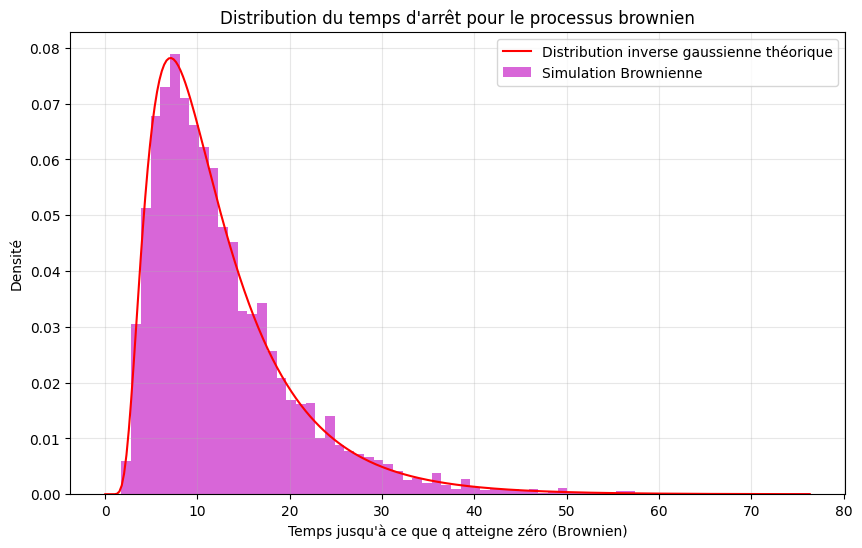
\includegraphics[width=\textwidth]{fig_ig.png}\\
{\scriptsize Densité IG théorique (rouge) vs histogramme simulé.}
\end{column}
\end{columns}
\end{frame}

%----------------------------------------------------------------
\begin{frame}{La probabilité de ruine, sans simuler}
\begin{columns}[T]
\begin{column}{0.46\textwidth}
Par conditionnement sur $\taua$ :
\[
\PP(\taua<\taub)=\int_0^\infty f_{\taua}(t)\,\bigl(1-F_{\taub}(t)\bigr)\,dt .
\]
Une simple quadrature de Gauss--Legendre remplace des millions de tirages.\\[1ex]
\textbf{Le point qui compte :} l'écart max à Monte-Carlo est $0{,}049$, soit exactement la barre d'erreur MC ($\approx 0{,}044$). \alert{Aucun biais} : la formule est exacte.
\end{column}
\begin{column}{0.54\textwidth}
\centering
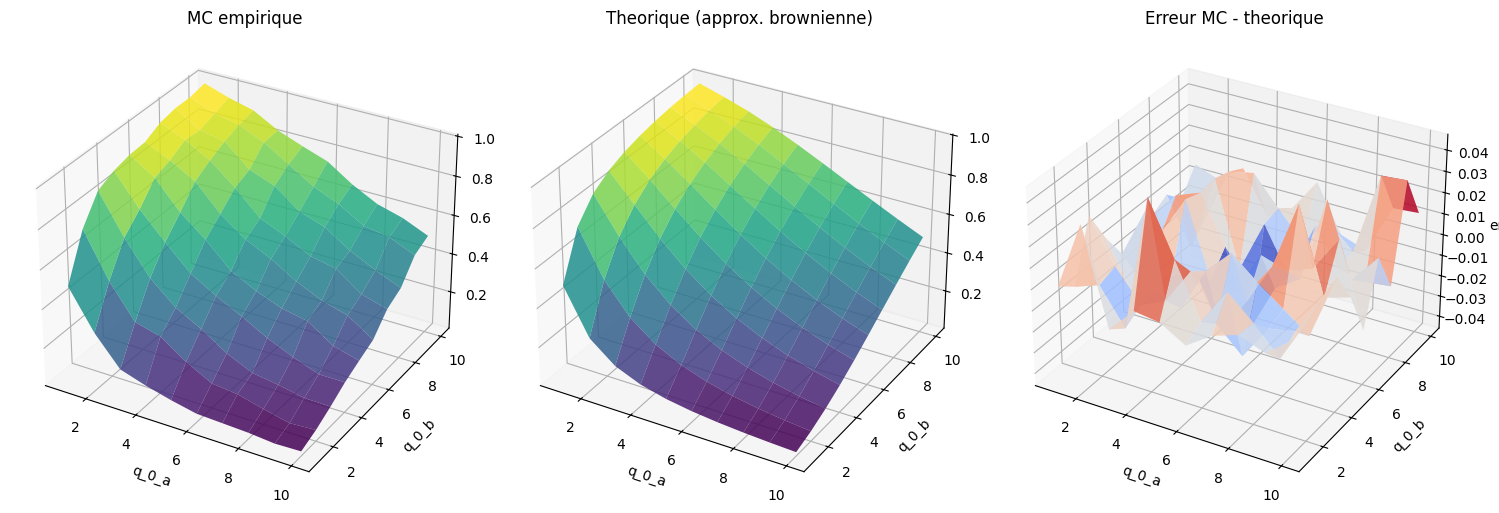
\includegraphics[width=\textwidth]{fig_ruine.png}\\
{\scriptsize MC (g.) vs quadrature IG (c.) vs écart (d.). Sur la diagonale $\hat p\approx\tfrac12$.}
\end{column}
\end{columns}
\end{frame}

%----------------------------------------------------------------
\begin{frame}{Ajouter la mémoire : Hawkes, et un piège numérique}
\begin{columns}[T]
\begin{column}{0.52\textwidth}
L'intensité d'annulation intègre la mémoire des événements passés :
\[
\lambda^-(t)=\mu^-+\alpha\!\!\sum_{s\in\mathcal N^-,\,s<t}\!\! e^{-\beta(t-s)}
-\alpha\!\!\sum_{s\in\mathcal N^+,\,s<t}\!\! e^{-\beta(t-s)}.
\]
{\scriptsize Chaque annulation ($\mathcal N^-$) excite $\lambda^-$ de $\alpha$ ; chaque insertion ($\mathcal N^+$) l'inhibe.}\\[0.3ex]
Théorie stationnaire : $\bar\lambda^-_\infty=2{,}80$.\\[0.5ex]
\textbf{Ce que la simulation révèle :} on mesure $2{,}96$, soit \alert{$+5{,}9\%$}. Pas du bruit.
\begin{block}{Le clipping fait le biais}
La mise à jour $\lambda^-\!\leftarrow\!\max(\lambda^-_{\text{pre}}-\alpha,0)$ tronque à zéro. Le bilan de flux supposé sur $\mathbb R$ est brisé : excès systématique.
\end{block}
\end{column}
\begin{column}{0.48\textwidth}
\centering
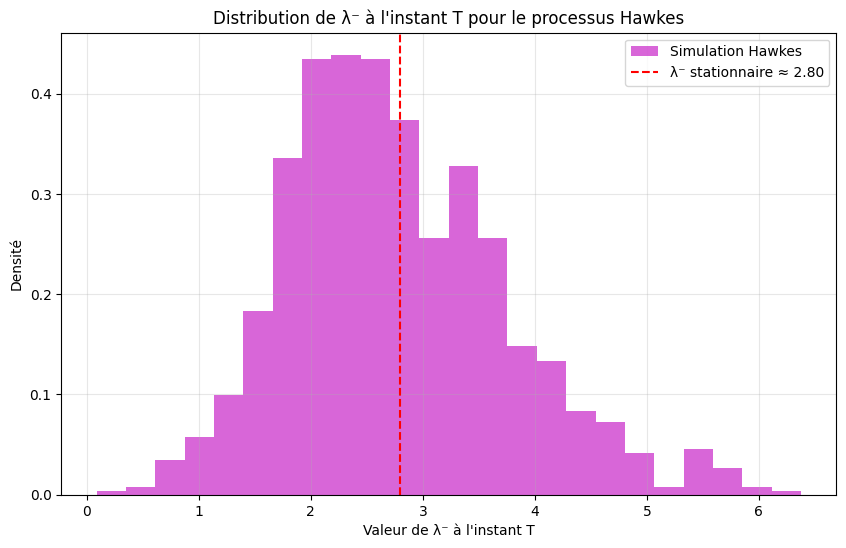
\includegraphics[width=\textwidth]{fig_hawkes_bias.png}\\
{\scriptsize Moyennes temporelles de $\lambda^-$ ; ligne rouge $=2{,}80$. La masse est décalée à droite.}
\end{column}
\end{columns}
\end{frame}

%----------------------------------------------------------------
\begin{frame}{Le couplage croisé : pourquoi un crash s'auto-alimente}
\begin{columns}[T]
\begin{column}{0.56\textwidth}
Auto-excitation par ses décréments, \alert{inhibition par ses incréments}, et excitation croisée par \emph{tout} événement de l'autre file :
\[
\resizebox{\linewidth}{!}{$\displaystyle
\lma(t)=\mu_a^- +\alpha\!\!\sum_{s\in\mathcal D_a}\!e^{-\beta(t-s)}
\,\alert{-\,\alpha\!\!\sum_{s\in\mathcal A_a}\!e^{-\beta(t-s)}}
\,+\alpha\!\!\sum_{s\in\mathcal C_b}\!e^{-\beta(t-s)}$}
\]
{\scriptsize $\mathcal D_a,\mathcal A_a$ : décréments / incréments ask ; $\mathcal C_b=\mathcal D_b\cup\mathcal A_b$ : tous les événements bid.}\\[1ex]
\textbf{Effet mesuré} (coin $q_0=10,10$) :
\[
\E[\min]:\; 8{,}3\ \text{(Poisson)}\ \to\ 5{,}8\ \text{(couplé)},\quad -30\%.
\]
Les deux côtés se vident \alert{ensemble} : c'est la signature microstructurale d'une cascade.
\end{column}
\begin{column}{0.44\textwidth}
\centering
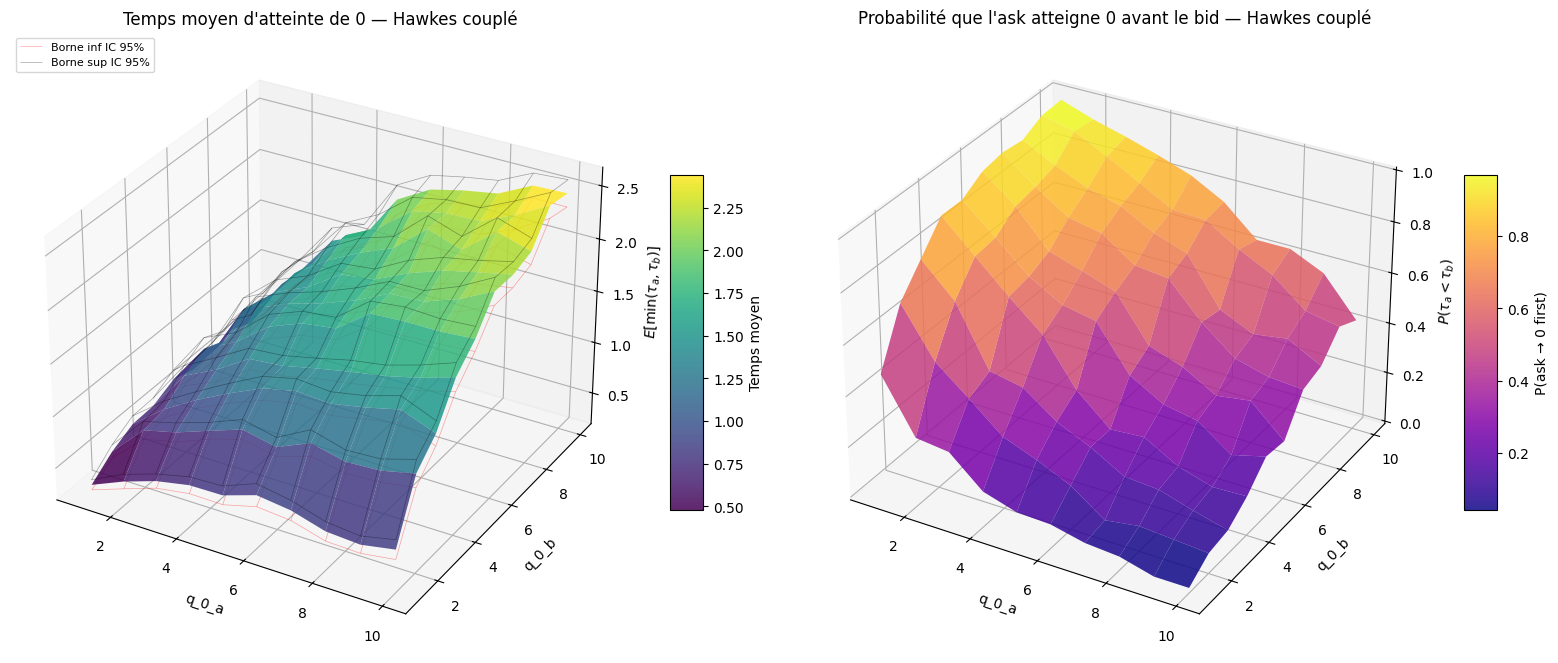
\includegraphics[width=\textwidth]{fig_couple3d.png}\\
{\scriptsize Hawkes couplé : $\E[\min(\taua,\taub)]$ (g.) et $\PP(\taua<\taub)$ (d.).}
\end{column}
\end{columns}
\end{frame}

%----------------------------------------------------------------
\begin{frame}{Quatre régimes, une tendance nette}
\begin{columns}[T]
\begin{column}{0.40\textwidth}
\centering
\small
\begin{tabular}{lcc}
\toprule
Modèle & Moy. & Méd.\\
\midrule
Poisson indiv. & 12{,}4 & 10{,}6\\
Min de 2 Poisson & 8{,}6 & 7{,}7\\
Hawkes indiv. & 8{,}8 & 6{,}9\\
\textbf{Hawkes couplé} & \textbf{5{,}9} & \textbf{5{,}1}\\
\bottomrule
\end{tabular}

\vspace{2ex}
\raggedright\normalsize
\textbf{L'idée à retenir :} la mémoire ne déplace pas seulement la moyenne, elle \alert{déforme toute la loi} — elle épaissit les extrêmes.
\end{column}
\begin{column}{0.58\textwidth}
\centering
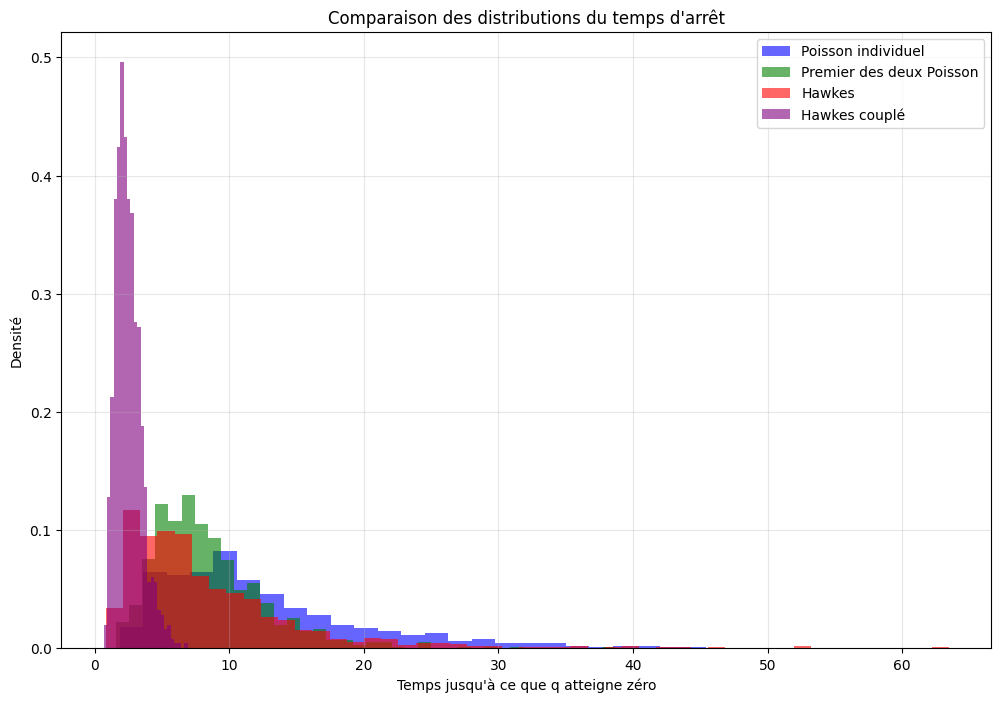
\includegraphics[width=0.92\textwidth]{fig_compare4.png}

\vspace{1ex}
\footnotesize\raggedright
Trois effets se cumulent : \textbf{(1)} prendre le minimum de deux files divise déjà la moyenne par $1{,}45$ — pur effet combinatoire ; \textbf{(2)} l'auto-excitation ajoute une queue gauche épaisse (les avalanches) ; \textbf{(3)} le couplage amplifie le tout, facteur global $\approx 2{,}1$.
\end{column}
\end{columns}
\end{frame}

%----------------------------------------------------------------
\begin{frame}{Avant le prix : le volume qui amorce le cycle}
\begin{columns}[T]
\begin{column}{0.40\textwidth}
Quand la première limite s'épuise, elle est aussitôt \alert{remplacée} par la deuxième. Le volume $q_2(\tau)$ présent à cet instant devient l'\emph{état initial} du cycle de prix qui suit.\\[1ex]

Il ne suffit donc pas d'une moyenne : on a besoin de toute sa \alert{loi conditionnelle}, et elle dépend du côté qui s'épuise.\\[1ex]

\textbf{Ce qu'on observe :} une loi en cloche décalée, de moyenne $\approx 7{,}7$ côté ask et $7{,}5$ côté bid — c'est cette distribution qu'on injectera dans la dynamique de prix.
\end{column}
\begin{column}{0.60\textwidth}
\centering
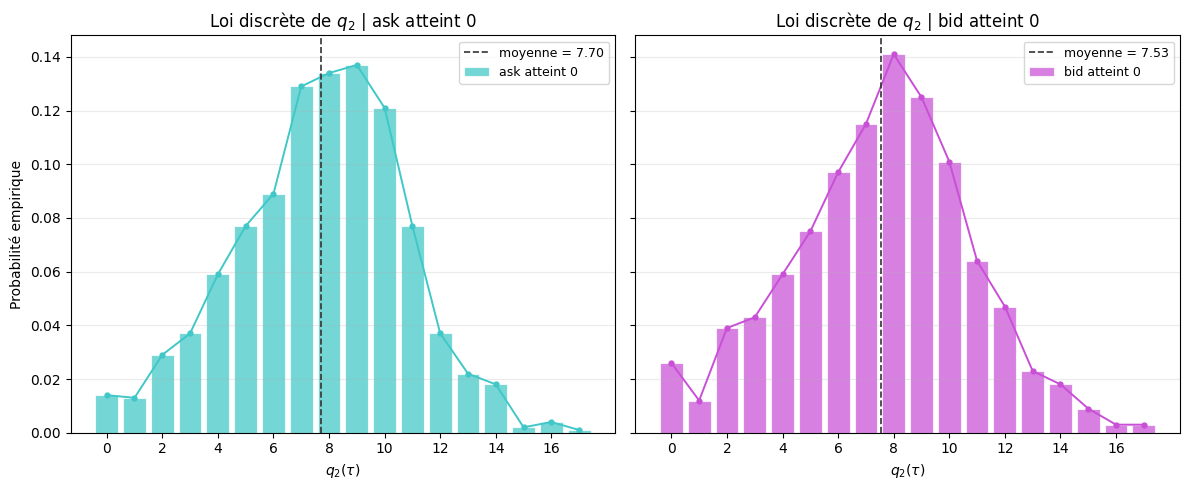
\includegraphics[width=\textwidth]{q2_cond.png}

\vspace{0.5ex}
{\footnotesize Loi conditionnelle de $q_2(\tau)$ selon le côté qui s'épuise (ask, g. ; bid, d.). Ligne pointillée : moyenne empirique.}
\end{column}
\end{columns}
\end{frame}

%----------------------------------------------------------------
\begin{frame}{Du volume au prix : une dérive identifiable}
\begin{columns}[T]
\begin{column}{0.42\textwidth}
Modèle à 4 limites : à chaque épuisement, le prix saute de $\pm\delta^p/2$, et les intensités Hawkes sont \alert{transportées} d'un cycle à l'autre.
\[
\Delta p_0=\tfrac{\delta^p}{2}(2p-1),\quad p=\PP(\taua<\taub).
\]
Le prix est une martingale $\iff p=\tfrac12 \iff \mu_a^-=\mu_b^-$.\\[1ex]
\textbf{L'enseignement :} en régime asymétrique, dérive prédite $0{,}238$, mesurée \alert{$0{,}2375$/cycle}. Observer la \emph{seule} dérive du prix suffit donc à inférer l'asymétrie cachée du carnet.
\end{column}
\begin{column}{0.58\textwidth}
\centering
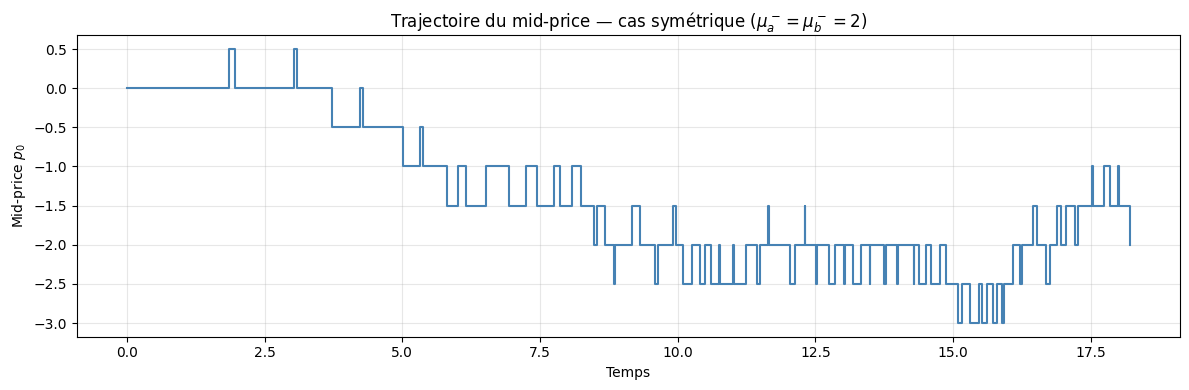
\includegraphics[width=\textwidth]{mp_sym.png}\\
{\scriptsize Cas symétrique : pas de tendance (martingale).}

\vspace{2.5ex}
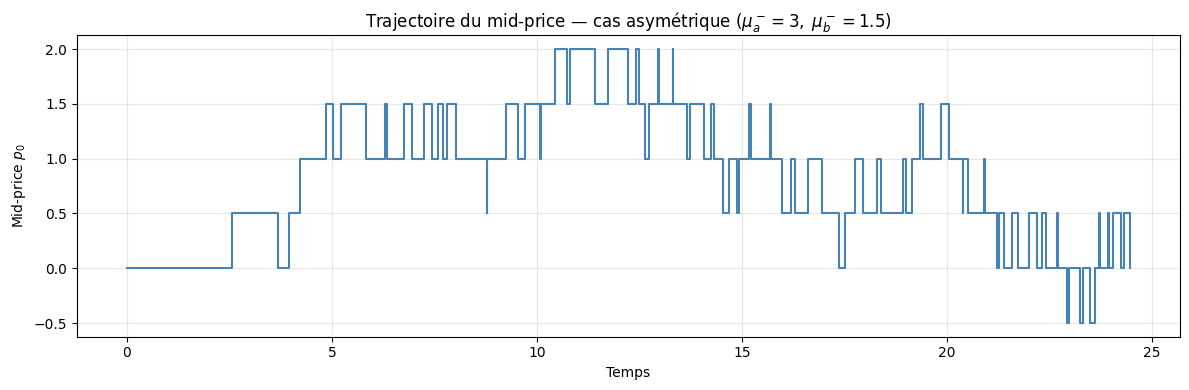
\includegraphics[width=\textwidth]{mp_asym.png}\\
{\scriptsize Cas asymétrique : tendance haussière nette.}
\end{column}
\end{columns}
\end{frame}

%================================================================
\xsection{red}[Partie II]{Estimer l'improbable}[beamerxbackground.jpg]

%----------------------------------------------------------------
\begin{frame}{Pourquoi le Monte-Carlo naïf est condamné}
\begin{columns}[T]
\begin{column}{0.55\textwidth}
\textbf{L'intuition.} Pour estimer une probabilité $p$, le Monte-Carlo compte les succès. Mais si l'événement n'arrive qu'une fois sur $10^{10}$ tirages\dots il faut tirer bien plus de $10^{10}$ fois pour en voir \emph{quelques-uns}.\\[1ex]

Formellement, la précision relative se dégrade en $\sqrt{1/(Mp)}$ : elle \alert{explose} quand $p\to 0$.\\[1ex]

\begin{itemize}
\item Cible visée : $p\sim 10^{-7}$ à $10^{-13}$.
\item Coût pour $10\%$ de précision : \alert{$10^{9}$ à $10^{15}$} trajectoires. Impraticable.
\end{itemize}
\end{column}
\begin{column}{0.45\textwidth}
\begin{block}{L'événement rare retenu}
L'épuisement du \emph{bid} alors qu'il est le côté le plus profond et le moins fragile ($\mu_a^->\mu_b^-$, $q_{b,0}>q_{a,0}$).\\[0.5ex]
C'est exactement le scénario d'un \alert{flash crash}, et c'est dur à atteindre par hasard.
\end{block}
\vspace{1ex}
\centering\footnotesize
Deux méthodes orthogonales, puis on les confronte.
\end{column}
\end{columns}
\end{frame}

%----------------------------------------------------------------
\begin{frame}{Splitting AMS : guider, palier par palier}
\begin{columns}[T]
\begin{column}{0.48\textwidth}
\textbf{L'intuition.} Plutôt que d'attendre qu'une trajectoire rare atteigne zéro par chance, on découpe la descente en \alert{paliers} de volume. À chaque palier, on jette les trajectoires qui reculent et on \alert{clone} celles qui progressent — en réinjectant leur état Hawkes complet.\\[1ex]

On guide ainsi l'effort de calcul exactement là où le Monte-Carlo naïf le gaspillerait.\\[1ex]

\textbf{Ce que la figure confirme :} l'écart-type décroît en $1/\sqrt N$ (pente log-log $\approx -0{,}5$). Le coefficient de variation chute d'un facteur $7$.
\end{column}
\begin{column}{0.52\textwidth}
\centering
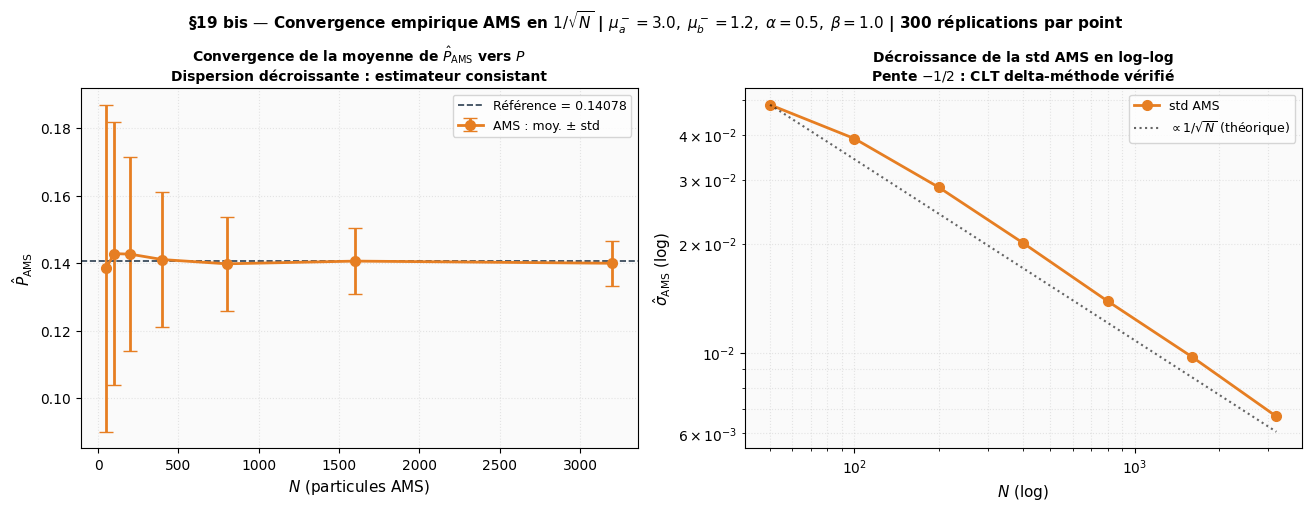
\includegraphics[width=\textwidth]{fig_ams_conv.png}

\vspace{0.5ex}
{\footnotesize Écart-type de $\hat P_{\text{AMS}}$ en fonction de $N$ : la droite log-log valide la CLT.}
\end{column}
\end{columns}
\end{frame}

%----------------------------------------------------------------
\begin{frame}{La loi de $Q_2$ : comment l'estimer efficacement ?}
\begin{columns}[T]
\begin{column}{0.40\textwidth}
On a vu en Partie I que la loi de $Q_{a,2}(\tau)$ amorce le cycle de prix. \alert{Comment l'estimer} ?\\[1ex]

Deux estimations indépendantes :
\begin{itemize}
\item \textbf{Monte-Carlo direct} (force brute).
\item \textbf{Splitting AMS} (machinerie par paliers).
\end{itemize}
\textbf{Verdict :} les deux lois se \alert{superposent} — l'AMS ne biaise pas la distribution conditionnelle, à coût bien moindre.
\end{column}
\begin{column}{0.60\textwidth}
\centering
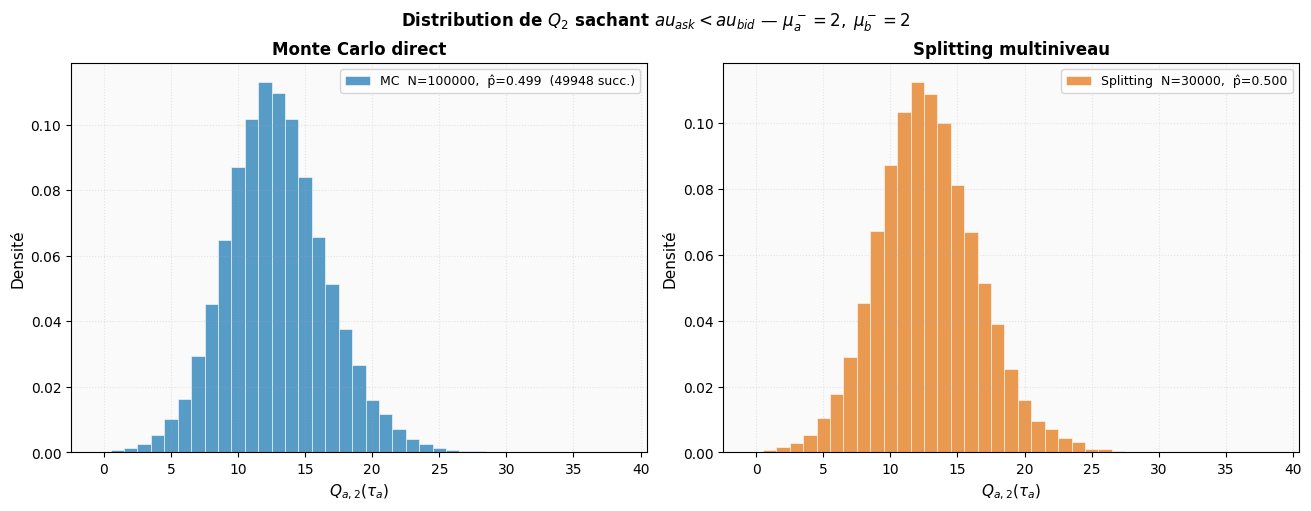
\includegraphics[width=\textwidth]{q2_mc_ams.png}

\vspace{0.5ex}
{\footnotesize Loi de $Q_{a,2}(\tau_a)$ : Monte-Carlo direct ($N{=}10^5$, g.) vs splitting AMS ($N{=}3\!\cdot\!10^4$, d.). Même forme, même support.}
\end{column}
\end{columns}
\end{frame}

%----------------------------------------------------------------
\begin{frame}{Splitting en deux phases : réutiliser $\hat\pi_{k^*}$}
\begin{columns}[T]
\begin{column}{0.40\textwidth}
\textbf{L'idée.} Les premiers paliers du splitting sont coûteux mais \alert{indépendants de la question finale}. On les calcule \emph{une fois}, hors-ligne, et on stocke la distribution empirique $\hat\pi_{k^*}$ des survivants.\\[1ex]

En ligne, on \alert{bootstrappe} depuis $\hat\pi_{k^*}$ et on ne simule que les derniers paliers :
\[
\hat P=\underbrace{\textstyle\prod_{j>k^*}\hat p_j}_{\text{hors-ligne}}\!\times\hat P(\cdot\mid q_{s,1}\!\le\! k^*).
\]
\textbf{Gain :} hors-ligne $7{,}7$\,s, puis chaque requête en ligne en $0{,}7$\,s — loi \emph{identique}.
\end{column}
\begin{column}{0.60\textwidth}
\centering
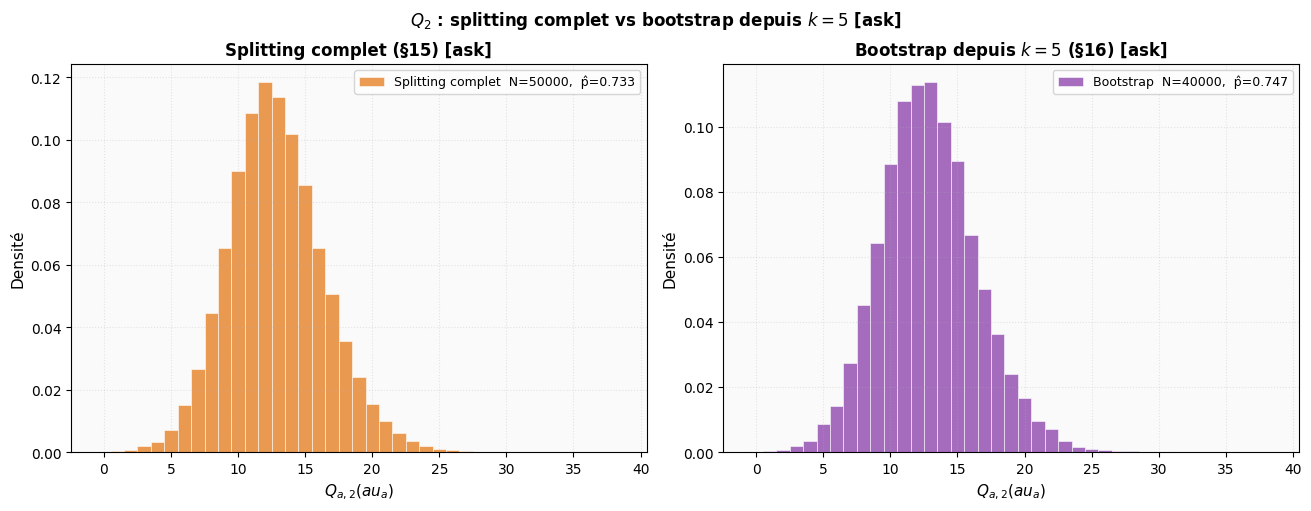
\includegraphics[width=\textwidth]{q2_boot.png}

\vspace{0.5ex}
{\footnotesize Loi de $Q_{a,2}$ : splitting complet (g.) vs bootstrap depuis $\hat\pi_{k^*=5}$ (d.). Moyennes $12{,}90$ vs $12{,}91$.}
\end{column}
\end{columns}
\end{frame}

%----------------------------------------------------------------
\begin{frame}{Importance sampling : utile, mais traître}
\begin{columns}[T]
\begin{column}{0.48\textwidth}
\textbf{L'intuition.} Au lieu de guider les trajectoires (AMS), on \alert{déforme la loi} pour rendre l'événement rare fréquent — puis on corrige le biais par un poids de vraisemblance. Le paramètre $\theta$ règle l'intensité de la déformation.\\[1ex]

\begin{itemize}
\item $\theta^*\approx 0{,}30$ : bon réglage, le CV baisse.
\item $\theta>0{,}6$ : les poids dégénèrent, \alert{le CV explose au-delà de $100$}.
\end{itemize}

\textbf{Le piège à voir :} à $\theta=2{,}1$ le CV \emph{rechute} — pas parce que l'estimateur s'améliore, mais parce que \alert{presque aucune trajectoire} n'atteint l'événement. Une faible variance peut cacher un estimateur mort.
\end{column}
\begin{column}{0.52\textwidth}
\centering
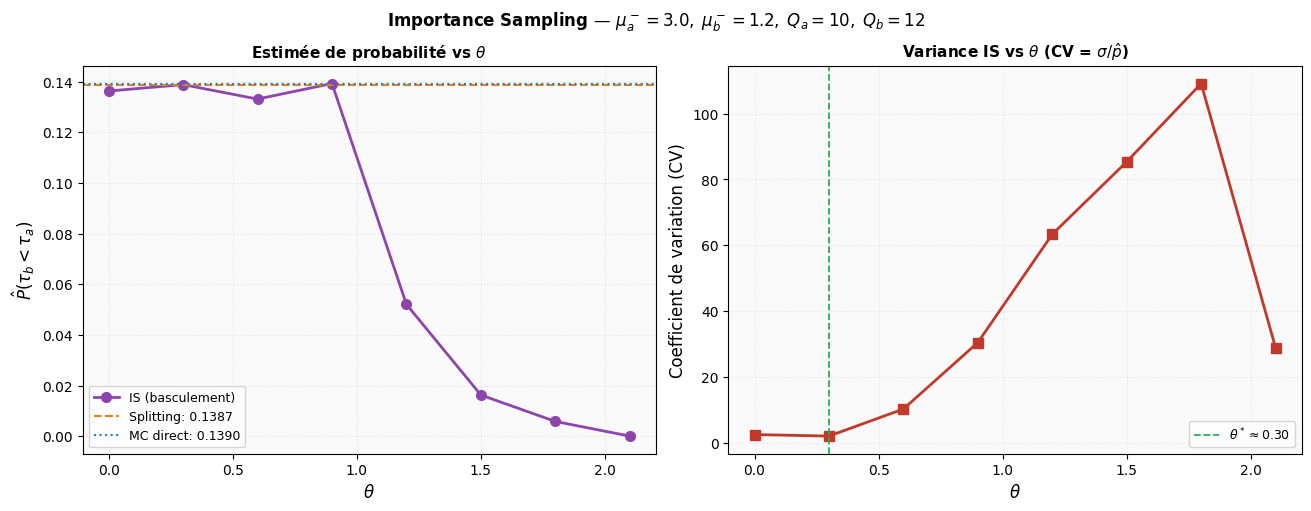
\includegraphics[width=\textwidth]{fig_is.png}

\vspace{0.5ex}
{\footnotesize Probabilité estimée (g.) et coefficient de variation (d.) en fonction de $\theta$ ; minimum net en $\theta^*\!\approx\!0{,}30$.}
\end{column}
\end{columns}
\end{frame}

%----------------------------------------------------------------
\begin{frame}{Verdict à $N$ fixé : un résultat contre-intuitif}
\centering
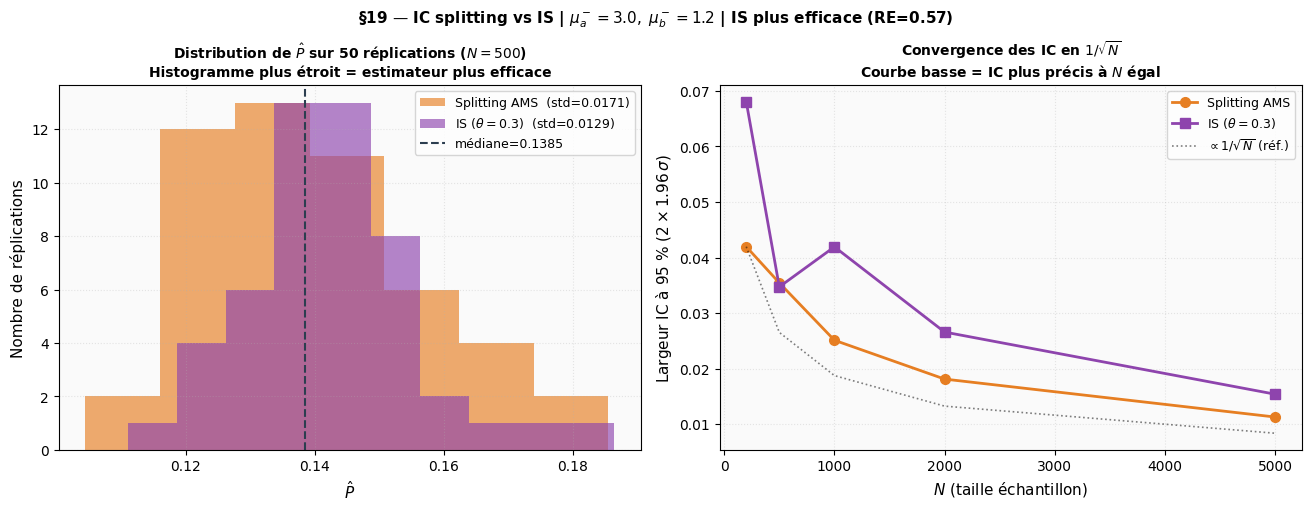
\includegraphics[width=0.78\textwidth]{fig_amsvis.png}

\vspace{0.3ex}
{\scriptsize À gauche : dispersion de $\hat P$ (le pic plus étroit de l'IS = variance moindre). À droite : largeur d'IC, en $1/\sqrt N$ pour les deux.}

\vspace{0.6ex}
\begin{columns}[c]
\begin{column}{0.26\textwidth}
\centering\scriptsize
\begin{tabular}{lc}
\toprule
 & RE\\
\midrule
AMS & $1{,}00$\\
IS ($\theta^*$) & \textbf{$0{,}57$}\\
\bottomrule
\end{tabular}
\end{column}
\begin{column}{0.70\textwidth}
\footnotesize
À $N$ égal, l'IS bien réglé \alert{bat} l'AMS ($-43\%$) — \emph{mais seulement en profondeur modérée}. Dès $k\ge 5$, l'AMS reprend la main. \alert{Le bon outil dépend de la profondeur du rare.}
\end{column}
\end{columns}
\end{frame}

%================================================================
\xsection{green}[Partie III]{Confronter au réel}[beamerxbackground.jpg]

%----------------------------------------------------------------
\begin{frame}{Calibration : retrouve-t-on les bons paramètres ?}
\centering
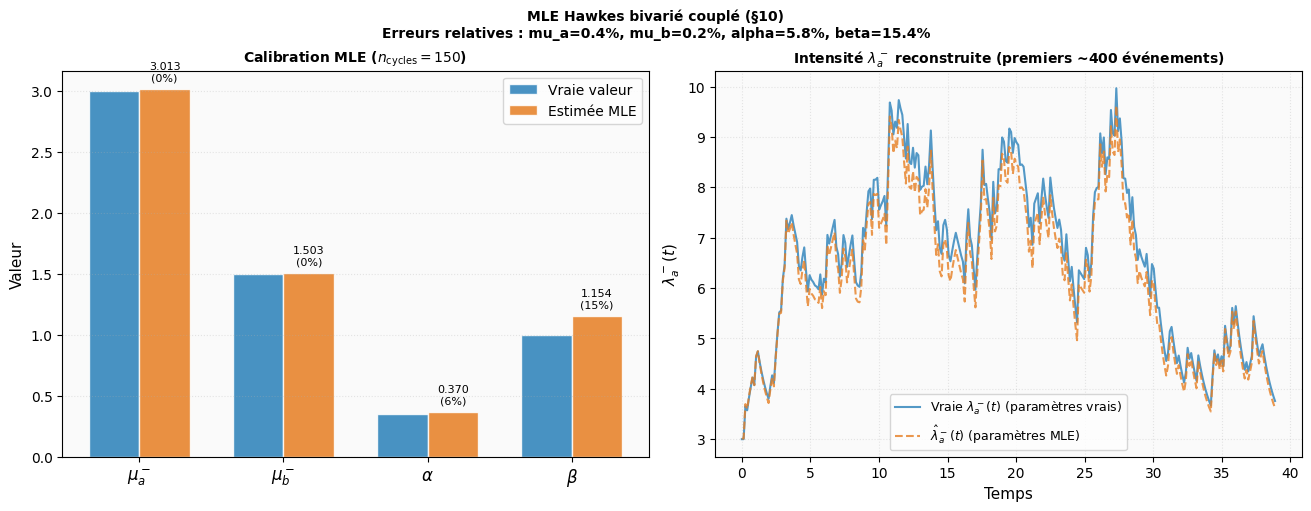
\includegraphics[width=0.80\textwidth]{cal_0.png}

\vspace{0.3ex}
{\scriptsize À gauche : vraies valeurs vs estimées MLE. À droite : intensité $\lambda_a^-(t)$ reconstruite (tirets) vs vraie (bleu).}

\vspace{0.8ex}
\begin{columns}[c]
\begin{column}{0.56\textwidth}
\footnotesize
\textbf{Validation synthétique (150 cycles).} On retrouve les \alert{fonds $\mu$ à moins de $1\%$} près. $(\alpha,\beta)$ sont plus bruités : fortement \emph{corrélés} dans la vraisemblance sur un échantillon court.
\end{column}
\begin{column}{0.42\textwidth}
\centering\scriptsize
\begin{tabular}{lcccc}
\toprule
 & $\mu_a^-$ & $\mu_b^-$ & $\alpha$ & $\beta$\\
\midrule
Vrai & 3{,}0 & 1{,}5 & 0{,}35 & 1{,}0\\
MLE & 3{,}01 & 1{,}50 & 0{,}37 & 1{,}15\\
Err. & $0\%$ & $0\%$ & $6\%$ & $15\%$\\
\bottomrule
\end{tabular}
\end{column}
\end{columns}
\end{frame}

%----------------------------------------------------------------
\begin{frame}{Black Thursday : le modèle rencontre le marché}
\centering
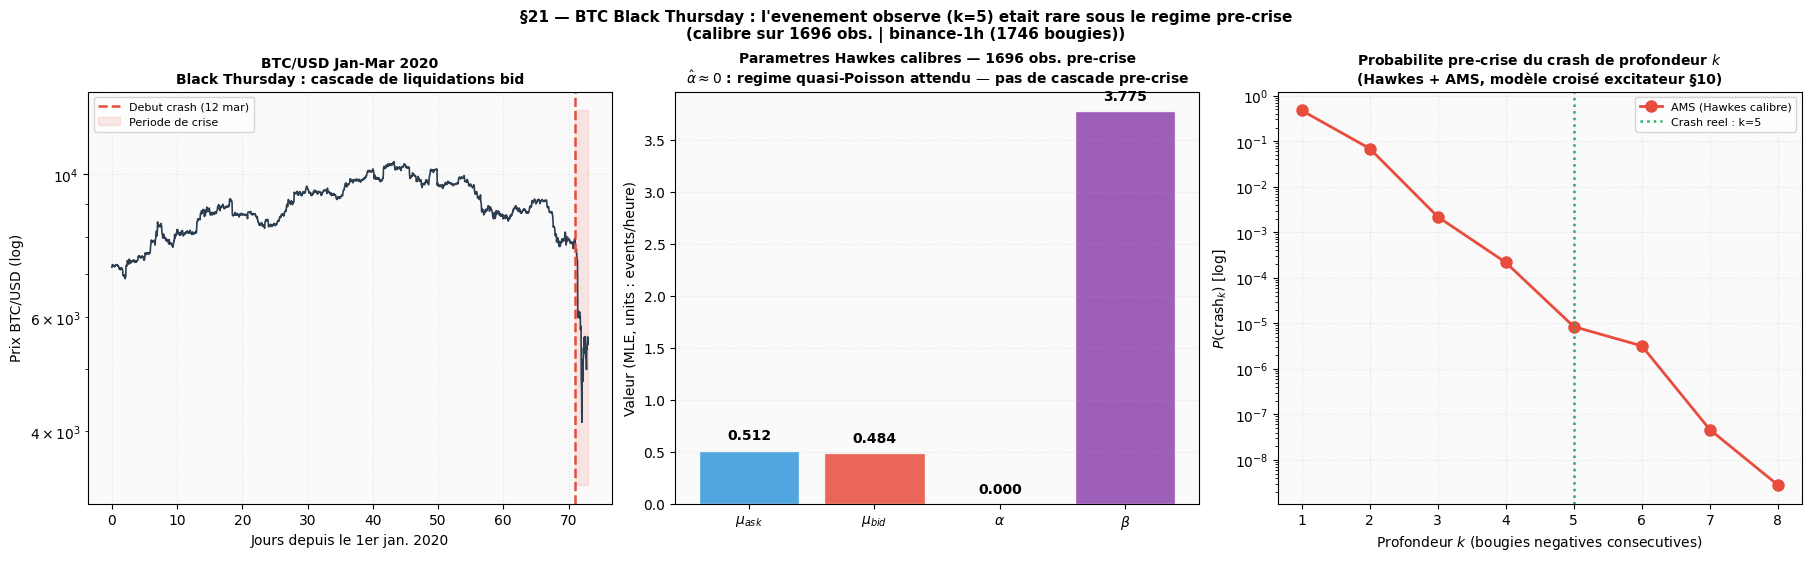
\includegraphics[width=0.96\textwidth]{fig_btc.png}\\[0.5ex]
\begin{columns}[T]
\begin{column}{0.5\textwidth}
\small
12 mars 2020 : BTC $-41\%$ en un jour. Bougies 1h Binance (1696 obs. pré-crise). Bougie négative $=$ décrément bid.
\end{column}
\begin{column}{0.5\textwidth}
\small
\textbf{Le punch :} le régime pré-crise est calibré \alert{$\hat\alpha\approx 0$} (quasi-Poisson, pas de mémoire). Sous ce régime, les 5 chutes consécutives observées avaient une proba AMS de \alert{$8{,}5\cdot 10^{-6}$} ($\approx 1/118\,000$). Le crash \emph{était} un événement rare — c'est précisément ce qu'on voulait quantifier.
\end{column}
\end{columns}
\end{frame}

%----------------------------------------------------------------
\begin{frame}{Ce qui n'a pas marché : GameStop}
\begin{block}{Une tentative abandonnée, et pourquoi c'est instructif}
On a voulu rejouer la même procédure sur le squeeze GME (janvier 2021, $\times 30$). Échec assumé :
\end{block}
\centering\small
\begin{tabular}{lll}
\toprule
& GME (journalier) & BTC (1h)\\
\midrule
Résolution & 70 obs. & 1696 obs.\\
Mécanisme & Coordination Reddit (\alert{exogène}) & Liquidations (\alert{endogène})\\
Calibration & Instable ($\hat\alpha\to 0$ ou $\beta^-$) & Stable\\
\bottomrule
\end{tabular}
\vspace{1.5ex}

\raggedright
\normalsize Deux leçons : (1) 70 points donnent une vraisemblance trop plate ; (2) surtout, le moteur de GME est \alert{hors du carnet} — notre modèle suppose un mécanisme endogène. Un bon modèle, c'est aussi savoir où il ne s'applique pas.
\end{frame}

%================================================================
\begin{frame}{Conclusion : trois charnières}
\begin{columns}[T]
\begin{column}{0.6\textwidth}
\begin{enumerate}
\item[\textbf{I.}] La \alert{mémoire déforme la loi} d'épuisement : $\E[\min]$ de $12{,}5\to 5{,}9$, et l'asymétrie devient lisible directement dans la dérive du prix.
\item[\textbf{II.}] Pour le \alert{rare}, AMS et IS sont complémentaires : l'IS gagne à $N$ fixé sur les événements modérés, l'AMS reste indispensable en profondeur.
\item[\textbf{III.}] Sur \alert{Black Thursday}, le modèle chiffre la rareté ($\sim 10^{-6}$) avec un régime pré-crise quasi-Poisson — et sait refuser GME.
\end{enumerate}
\end{column}
\begin{column}{0.4\textwidth}
\begin{block}{Perspectives}
\begin{itemize}
\item Données tick-by-tick (TARDIS/Kaiko) pour mieux séparer $\alpha,\beta$.
\item Extension à $L>2$ niveaux.
\item Relier $\PP(\taua<\taub)$ à une surface de volatilité implicite.
\end{itemize}
\end{block}
\end{column}
\end{columns}
\vspace{1ex}
\centering \rmfamily\large\color{bleu303} Merci --- questions ?
\end{frame}

\end{document}
